\documentclass[12pt,a4paper]{article}

% ─── Page Layout ───────────────────────────────────────────────────────────────
\usepackage[a4paper, margin=0.8in, headheight=14pt]{geometry}

% ─── Fonts (XeLaTeX) ───────────────────────────────────────────────────────────
\usepackage{fontspec}
\usepackage{unicode-math}
\setmainfont{TeX Gyre Pagella}
\setmonofont[Scale=0.88]{TeX Gyre Cursor}
\setmathfont{Latin Modern Math}

% ─── Packages ──────────────────────────────────────────────────────────────────
\usepackage{xcolor}
\usepackage{colortbl}
\usepackage{titlesec}
\usepackage{enumitem}
\usepackage{tabularx}
\usepackage{longtable}
\usepackage{booktabs}
\usepackage{array}
\usepackage{amsmath}
\usepackage{tikz}
\usetikzlibrary{shapes.geometric, arrows.meta, positioning, calc, fit, decorations.pathreplacing, patterns}
\usepackage{tcolorbox}
\tcbuselibrary{skins, breakable}
\usepackage{hyperref}
\usepackage{fancyhdr}
\usepackage{graphicx}
\usepackage{microtype}
\hyphenpenalty=10000
\exhyphenpenalty=10000
\sloppy
\usepackage{caption}
\usepackage{setspace}
\usepackage{multirow}
\usepackage{tocloft}

% ─── Q&A helper ────────────────────────────────────────────────────────────────
\newcommand{\Q}[1]{\textbf{#1}\par\noindent\ignorespaces}

% ─── Colour Palette ────────────────────────────────────────────────────────────
\definecolor{myred}{RGB}{196,30,58}
\definecolor{mydark}{RGB}{30,30,50}
\definecolor{mygreen}{RGB}{14,120,80}
\definecolor{myteal}{RGB}{0,130,140}
\definecolor{myamber}{RGB}{180,100,0}
\definecolor{mypurple}{RGB}{100,30,160}
\definecolor{mygray}{RGB}{246,247,249}
\definecolor{mgframe}{RGB}{180,185,200}
\definecolor{watermark}{RGB}{145,150,170}
\definecolor{hdrred}{RGB}{250,232,235}
\definecolor{hdrgreen}{RGB}{220,244,233}
\definecolor{hdrteal}{RGB}{220,242,244}
\definecolor{hdramber}{RGB}{253,242,215}
\definecolor{hdrpurple}{RGB}{238,228,255}
\definecolor{hdrgray}{RGB}{238,240,245}

% ─── Section Formatting ────────────────────────────────────────────────────────
\titleformat{\section}
  {\large\bfseries\color{myred}}{\thesection.}{0.5em}{}
  [\vspace{1pt}{\color{myred}\rule{\linewidth}{0.8pt}}]
\titleformat{\subsection}
  {\normalsize\bfseries\color{myteal}}{\thesubsection}{0.5em}{}
\titlespacing*{\section}{0pt}{18pt}{7pt}
\titlespacing*{\subsection}{0pt}{11pt}{4pt}

% ─── Paragraph ─────────────────────────────────────────────────────────────────
\setlength{\parindent}{0pt}
\setlength{\parskip}{4pt}

% ─── TOC Styling ───────────────────────────────────────────────────────────────
\renewcommand{\cfttoctitlefont}{\large\bfseries\color{myred}}
\renewcommand{\cftaftertoctitle}{\par\noindent{\color{myred}\rule{\linewidth}{0.8pt}}}
\setlength{\cftbeforetoctitleskip}{0pt}
\setlength{\cftaftertoctitleskip}{6pt}
\renewcommand{\cftsecfont}{\normalsize\bfseries\color{mydark}}
\renewcommand{\cftsecpagefont}{\normalsize\bfseries\color{mydark}}
\renewcommand{\cftsecleader}{\cftdotfill{\cftdotsep}}
\setlength{\cftbeforesecskip}{7pt}
\renewcommand{\cftsubsecfont}{\small\color{mydark}}
\renewcommand{\cftsubsecpagefont}{\small\color{mydark}}
\setlength{\cftbeforesubsecskip}{3pt}
\setlength{\cftsubsecindent}{1.4em}

% ─── Table helpers ─────────────────────────────────────────────────────────────
\renewcommand{\arraystretch}{1.45}
\setlength{\tabcolsep}{6pt}
\arrayrulecolor{mydark}
\newcolumntype{B}[1]{>{\small\bfseries\raggedright\arraybackslash}m{#1}}
\newcolumntype{Y}{>{\small\raggedright\arraybackslash}X}
\renewcommand{\tabularxcolumn}[1]{m{#1}}

% ─── Header / Footer ───────────────────────────────────────────────────────────
\pagestyle{fancy}
\fancyhf{}
\fancyhead[L]{\small\color{myred}\textbf{BS-B401}\;\color{mydark}--- Biology for Engineers}
\fancyhead[R]{\small\color{myteal}\textbf{Module 1 Notes}}
\fancyfoot[C]{\small\color{mydark}\thepage}
\fancyfoot[R]{\small\color{watermark}\textit{\copyright\ Biraj Sarkar (CGEC)}}
\renewcommand{\headrulewidth}{0.5pt}
\renewcommand{\footrulewidth}{0.3pt}

% ─── Hyperref ──────────────────────────────────────────────────────────────────
\hypersetup{
  colorlinks=true, linkcolor=myteal, urlcolor=myteal,
  pdfauthor={Biraj Sarkar (CGEC)},
  pdftitle={BS-B401 --- Module 1 Notes: Biology and Engineering}
}

% ─── tcolorbox styles ──────────────────────────────────────────────────────────
\tcbset{
  tikzbox/.style={
    colback=mygray, colframe=mgframe, boxrule=0.6pt, arc=4pt,
    left=8pt, right=8pt, top=6pt, bottom=6pt,
    colbacktitle=mgframe, coltitle=mydark, fonttitle=\small\bfseries
  },
  defbox/.style={
    colback=hdrgreen, colframe=mygreen, boxrule=0.8pt, arc=4pt,
    left=9pt, right=9pt, top=6pt, bottom=6pt,
    colbacktitle=mygreen, coltitle=white, fonttitle=\small\bfseries
  },
  formulabox/.style={
    colback=hdrteal, colframe=myteal, boxrule=0.8pt, arc=4pt,
    left=9pt, right=9pt, top=7pt, bottom=7pt,
    colbacktitle=myteal, coltitle=white, fonttitle=\small\bfseries
  },
  examplebox/.style={
    colback=hdramber, colframe=myamber, boxrule=0.8pt, arc=4pt,
    left=9pt, right=9pt, top=6pt, bottom=6pt,
    colbacktitle=myamber, coltitle=white, fonttitle=\small\bfseries
  },
  masonbox/.style={
    colback=hdrpurple, colframe=mypurple, boxrule=0.8pt, arc=4pt,
    left=9pt, right=9pt, top=6pt, bottom=6pt,
    colbacktitle=mypurple, coltitle=white, fonttitle=\small\bfseries
  },
  exambox/.style={
    colback=hdrpurple, colframe=mypurple, boxrule=1pt, arc=5pt,
    left=10pt, right=10pt, top=8pt, bottom=8pt,
    colbacktitle=mypurple, coltitle=white, fonttitle=\bfseries,
    breakable, title after break={\textbf{Frequently Asked / Viva Questions (contd.)}}
  }
}
\tcbset{breakable}
\tcbset{after={\par\color{black}}}

% ─── TikZ styles ───────────────────────────────────────────────────────────────
\tikzset{
  block/.style={rectangle, draw=myteal, fill=hdrteal,
    text width=2.4cm, align=center, minimum height=0.95cm,
    font=\small, rounded corners=3pt, line width=0.7pt},
  redblock/.style={rectangle, draw=myred, fill=hdrred,
    text width=2.4cm, align=center, minimum height=0.95cm,
    font=\small, rounded corners=3pt, line width=0.7pt},
  amberblock/.style={rectangle, draw=myamber, fill=hdramber,
    text width=2.4cm, align=center, minimum height=0.95cm,
    font=\small, rounded corners=3pt, line width=0.7pt},
  sumjunc/.style={circle, draw=myamber, fill=hdramber,
    minimum size=0.62cm, font=\small, line width=0.8pt},
  arrow/.style={-Stealth, thick, color=mydark},
  redarrow/.style={-Stealth, thick, color=myred},
  line/.style={thick, color=mydark}
}

\begin{document}

% ─── Title Page ───────────────────────────────────────────────────────────────
\begin{center}
  {\LARGE\bfseries\color{myred} BS-B401 --- Biology for Engineers}\\[5pt]
  {\normalsize\color{mydark} Semester IV \quad$\bullet$\quad 2L:1T:0P \quad$\bullet$\quad 3 Credits}\\[3pt]
  {\normalsize\color{myteal}\textbf{Module 1 Exam Notes: Biology and Engineering}}\\[3pt]
  {\small\color{mydark} CGEC \;$|$\; B.Tech ECE (2023--27) \;$|$\; \textit{Biraj Sarkar}}
\end{center}
\vspace{2pt}
\noindent{\color{myred}\rule{\linewidth}{1.5pt}}
\vspace{2pt}

\hypersetup{linkcolor=mydark}
\tableofcontents
\hypersetup{linkcolor=myteal}
\newpage

\section{Biology and Engineering}
\subsection{How science and engineering ask different questions}
\begin{tcolorbox}[defbox, title={Biology}]
Biology is the scientific study of living systems. It asks how organisms are built, how they work, how they inherit characteristics, and how they interact and evolve. It uses evidence and quantitative reasoning alongside physics, chemistry and mathematics.
\end{tcolorbox}

\par\vspace{5pt}
\begingroup
\setlength{\extrarowheight}{1pt}
\noindent\begin{tabularx}{\linewidth}{|B{3cm}|Y|Y|}
\hline
\textbf{Question} & \textbf{Scientific approach} & \textbf{Engineering approach} \\ \hline
Purpose & Explain and predict a natural phenomenon. & Design a solution that meets a specified need. \\ \hline
Starting point & Observe a pattern and form a testable hypothesis. & Set a goal, performance criteria and constraints. \\ \hline
Evidence & Compare predictions with measurements, controls and repeated observations. & Test a prototype against requirements for performance, cost, reliability or safety. \\ \hline
Outcome & A model that may be revised when new evidence arrives. & A design that may be revised when tests reveal a weakness. \\ \hline
\end{tabularx}\par
\endgroup
\begin{itemize}[leftmargin=*, itemsep=3pt, topsep=4pt]
  \item \textbf{Overlap.} An engineer uses scientific laws to design a system. A biologist uses engineered tools such as microscopes and sensors to collect evidence.
  \item \textbf{Why biology matters.} Biological systems sense, process information, use energy and adapt. Engineers encounter these ideas in imaging, biomechanics, environmental monitoring and sustainable material design.
  \item \textbf{What makes it distinctive.} Living systems retain information across generations while varying and evolving. Interactions among components can produce a system-level property, such as coordinated movement, that individual cells cannot produce alone.
\end{itemize}
\subsection{Eye and camera}
\begin{tcolorbox}[tikzbox, title={Two imaging chains}]
\centering
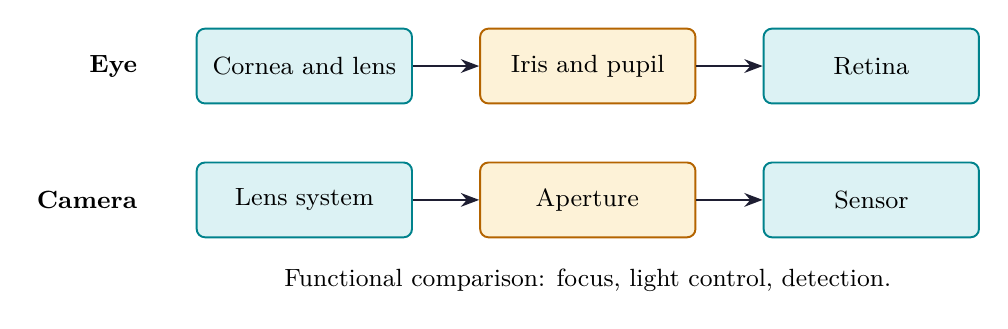
\begin{tikzpicture}[every node/.style={font=\small}]
\foreach \yy/\tag/\focus/\control/\detect in {1.3/Eye/{Cornea and lens}/{Iris and pupil}/{Retina},-0.4/Camera/{Lens system}/{Aperture}/{Sensor}} {
  \node[anchor=east,font=\small\bfseries] at (0,\yy) {\tag};
  \node[block,text width=2.5cm] (a) at (2,\yy) {\focus};
  \node[amberblock,text width=2.5cm] (b) at (5.6,\yy) {\control};
  \node[block,text width=2.5cm] (c) at (9.2,\yy) {\detect};
  \draw[arrow] (a)--(b);
  \draw[arrow] (b)--(c);
}
\node[align=center] at (5.6,-1.42) {Functional comparison: focus, light control, detection.};
\end{tikzpicture}\par
\end{tcolorbox}

\par\vspace{5pt}
\begingroup
\setlength{\extrarowheight}{1pt}
\noindent\begin{tabularx}{\linewidth}{|B{3cm}|Y|Y|}
\hline
\textbf{Function} & \textbf{Human eye} & \textbf{Camera} \\ \hline
Focus & The cornea supplies much of the refraction. Accommodation changes lens shape. & Lens elements focus the image, commonly by moving relative to each other or the sensor. \\ \hline
Control light & The iris changes pupil diameter. Photoreceptors also adapt to light level. & The aperture sets the light opening. Exposure time also controls the collected light. \\ \hline
Detect the image & Rods and cones respond to light. Retinal circuits and the brain process the signals. & Sensor pixels convert light into electrical signals. Electronics record and process the image. \\ \hline
\end{tabularx}\par
\endgroup
\begin{tcolorbox}[masonbox, title={State the limits of the analogy}]
The comparison is functional. The pupil is an opening controlled by the iris. The retina is living neural tissue, while the camera sensor is a manufactured detector. The diagram groups functions rather than showing anatomical order.
\end{tcolorbox}

\subsection{Bird flight and an aircraft}
\begin{itemize}[leftmargin=*, itemsep=3pt, topsep=4pt]
  \item \textbf{Lift.} Bird wings and aircraft wings generate aerodynamic forces as air flows around them. In steady, level, unaccelerated flight, the upward force balances weight.
  \item \textbf{Thrust and drag.} Flapping wings can provide thrust as well as lift. A typical powered fixed-wing aircraft uses a propeller or jet for thrust. In steady level flight, thrust balances drag in the flight direction.
  \item \textbf{Control.} Birds vary wing shape, feathers and tail position. Aircraft may use ailerons, elevators, rudders or other control surfaces.
  \item \textbf{Design lesson.} A natural flyer shows useful principles. An aircraft designer still tests the chosen geometry against load, energy use and stability requirements.
\end{itemize}
\section{How Biological Observations Lead to Discoveries}
\begin{enumerate}[leftmargin=*, itemsep=3pt, topsep=4pt]
  \item \textbf{Observe.} Describe what is seen and under which conditions.
  \item \textbf{Compare.} Deliberately vary a factor or use a comparison case to rule out alternatives.
  \item \textbf{Explain and test.} A proposed cause must predict further outcomes. Later experiments can separate competing explanations.
\end{enumerate}
\begin{tcolorbox}[examplebox, title={An eighteenth-century example: Ingenhousz}]
In 1779, Jan Ingenhousz compared plant effects on air in light and darkness. In sunlight the green portions improved the air by releasing oxygen. Comparing illuminated and shaded material connected the effect to light and green tissues, helping establish a basis for the study of photosynthesis.
\end{tcolorbox}

\begin{tcolorbox}[examplebox, title={Robert Brown and irregular particle motion}]
\begin{itemize}[leftmargin=*, itemsep=3pt, topsep=4pt]
  \item In 1827 Brown observed persistent irregular movement of minute particles suspended in water while examining material from pollen.
  \item He saw similar motion in particles from non-living materials. The comparison showed that the motion did not require living pollen.
  \item The later molecular account explains the random movement as the effect of unequal impacts by moving molecules of the surrounding fluid. Brown recorded the observation in 1828.
\end{itemize}
\end{tcolorbox}

\begin{tcolorbox}[examplebox, title={Julius Robert Mayer and energy conservation}]
\begin{itemize}[leftmargin=*, itemsep=3pt, topsep=4pt]
  \item Mayer noticed unusually bright venous blood while working as a physician in a tropical setting. He considered how different heat demands might affect oxygen use.
  \item The observation inspired a broader question: how are chemical processes, body heat and mechanical work related?
  \item In 1842 he published an early account of the conversion of mechanical work and heat and the conservation of what we now call energy. The observation prompted the idea. Quantitative arguments and experiments were needed to develop the general principle.
\end{itemize}
\end{tcolorbox}

\begin{tcolorbox}[masonbox, title={Exam chronology}]
Use Ingenhousz for the eighteenth century. Brown's observations and Mayer's publication belong to the nineteenth century. The syllabus's Julius Mayor refers to Julius Robert Mayer.
\end{tcolorbox}

\textbf{Primary readings.} \href{https://www.biodiversitylibrary.org/item/127139}{Ingenhousz (1779)}, \href{https://www.rpgroup.caltech.edu/marseillePBoC2024/assets/pdfs/Brown1828.pdf}{Brown (1828)}, and \href{https://web.lemoyne.edu/Giunta/mayer.html}{Mayer (1842, English translation)}.

\subsection{From biological observation to an engineering model}
\begin{tcolorbox}[examplebox, title={Work the eye--camera analogy with a thin lens}]
An object lies $120\,\mathrm{mm}$ in front of a converging camera lens of focal length $24\,\mathrm{mm}$. Use positive distances for this real object and real image.
\[
\begin{aligned}
\frac1v&=\frac1f-\frac1u
=\frac1{24}-\frac1{120}
=\frac1{30}\,\mathrm{mm}^{-1},\\
v&=30\,\mathrm{mm}.
\end{aligned}
\]
For a very distant object, $1/u\approx0$, so the image forms about $24\,\mathrm{mm}$ behind the lens. In the simple camera model, focusing nearer changes the required lens-to-sensor distance. A human eye accommodates by changing lens shape and optical power while the retina's location is approximately fixed.
\end{tcolorbox}

\begin{tcolorbox}[examplebox, title={Turn the flight comparison into a design problem}]
For a $2.0\,\mathrm{kg}$ model aircraft in steady, level flight, assume its wings provide the upward force. Required lift is $L=mg=2.0(9.81)\approx19.6\,\mathrm N$. A bird of the same mass needs the same average vertical support under these conditions. Its moving wings can also generate thrust, so the instantaneous forces vary through a wingbeat. A design team would measure average lift, power and stability separately before choosing a flapping or fixed-wing design.
\end{tcolorbox}

\subsection{What makes an explanation convincing?}
\begin{enumerate}[leftmargin=*, itemsep=2pt]
  \item \textbf{Separate observation and explanation.} Brown observed irregular displacements. Molecular collisions provide a later explanation.
  \item \textbf{Predict a difference.} A steady current would make many nearby particles drift systematically in the same direction. In still fluid, random displacements have no preferred direction.
  \item \textbf{Use repeated observations.} One trajectory can be misleading. Comparing many trajectories helps distinguish a consistent drift from irregular motion.
  \item \textbf{State the limit.} Brown's non-living comparison ruled out a requirement for living particles. Mayer's observation likewise raised an energy question that needed a separate physical argument.
\end{enumerate}

\newpage
\begin{center}
  {\large\bfseries\color{myred} Quick Revision --- Module 1}\\[3pt]
  {\small\color{mydark} Biology and Engineering $|$ BS-B401}
\end{center}
\noindent{\color{myred}\rule{\linewidth}{1.2pt}}\par\vspace{4pt}

\begin{tcolorbox}[formulabox, title={Key Concepts at a Glance}]
\renewcommand{\arraystretch}{1.35}
\noindent\begin{tabularx}{\linewidth}{B{4.5cm}Y}
Science & Explain a natural pattern using testable predictions. \\[3pt]
Engineering & Design and test a solution against requirements. \\[3pt]
Level flight & Lift balances weight and thrust balances drag in steady level flight. \\[3pt]
\end{tabularx}\par
\end{tcolorbox}

\begin{tcolorbox}[defbox, title={One-Line Definitions}]
\begin{itemize}[leftmargin=*, itemsep=3pt, topsep=4pt]
  \item \textbf{Hypothesis.} A testable proposed explanation.
  \item \textbf{Biomimetics.} Engineering inspired by structures or processes in living systems.
  \item \textbf{Brownian motion.} Irregular movement of small suspended particles.
\end{itemize}
\end{tcolorbox}

\begin{tcolorbox}[exambox, title={Frequently Asked / Viva Questions}]
\begin{enumerate}[topsep=0pt, label=\textbf{Q\arabic*.}, itemsep=5pt, leftmargin=*]
  \item \Q{What does biology study?}
    The structure, function, heredity, evolution and interactions of living systems.
  \item \Q{How do scientists test a proposed cause?}
    Compare predictions with measurements and use controls where possible.
  \item \Q{How is an engineering design evaluated?}
    Check its measured performance against the specified requirements.
  \item \Q{What controls pupil diameter?}
    The iris.
  \item \Q{Where is an image detected in the eye?}
    At the retina, where photoreceptors respond to light.
  \item \Q{How can a bird generate thrust?}
    Flapping can push air backwards and generate forward force.
  \item \Q{What did Ingenhousz compare?}
    Plant effects on air in light and darkness.
  \item \Q{How did Brown test whether the motion needed life?}
    He compared material from living sources with non-living particles.
  \item \Q{What question did Mayer's observation prompt?}
    How chemical energy use, heat and work are related.
  \item \Q{When were the three observations reported?}
    Ingenhousz in 1779, Brown in 1828 and Mayer's energy paper in 1842.
\end{enumerate}
\end{tcolorbox}

\begin{tcolorbox}[tikzbox, title={Summary Comparison}]
\par\vspace{5pt}
\begingroup
\setlength{\extrarowheight}{1pt}
\noindent\begin{tabularx}{\linewidth}{|B{3.45cm}|Y|Y|}
\hline
\textbf{Example} & \textbf{Scientific question} & \textbf{Engineering use} \\ \hline
Eye and camera & How does biological vision detect light? & Design focusing, exposure and detection systems. \\ \hline
Bird and aircraft & How do wing motion and shape affect flight? & Design lifting surfaces, propulsion and stability controls. \\ \hline
\end{tabularx}\par
\endgroup
\end{tcolorbox}

\end{document}
